\chapter{Wykład 4. Zarządzanie wiedzą w przedsiębiorstwach}

\section{Procesy wykorzystania produktu projektu}
% strona 34

\begin{figure}[hbt]
\centering
\includegraphics[width=0.6\textwidth]{opracowanieWBS.png}
\caption{Tworzenie WBS}
\label{fig:opracowanieWBS}
\end{figure}

\begin{figure}[hbt]
\centering
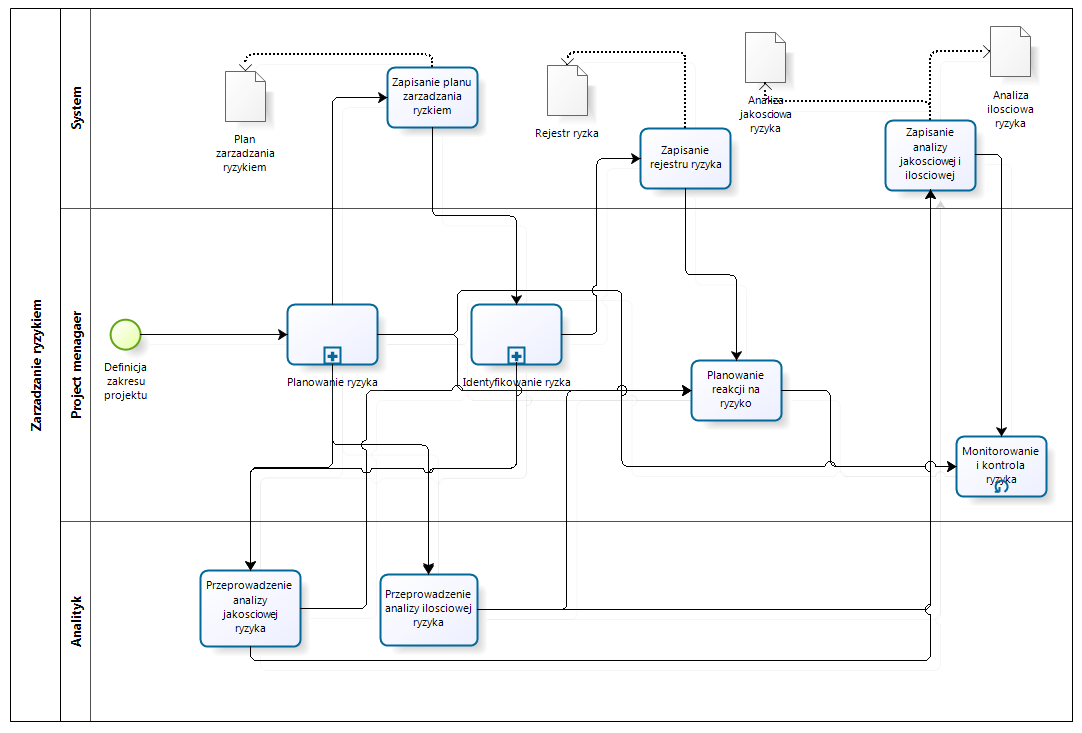
\includegraphics[width=0.6\textwidth]{zarzadzanieRyzykiem.png}
\caption{Zarządzanie ryzykiem}
\label{fig:zarzadzanieRyzykiem}
\end{figure}

% ===========================================================================

\section{Model przepływu danych}
% strona 40

Ten wirtualny warsztat jest beznadziejny.

% ===========================================================================

\section{Mapa umysłu dla systemu zarządzania wiedzą}
% strona 70

\begin{figure}[hbt]
\centering
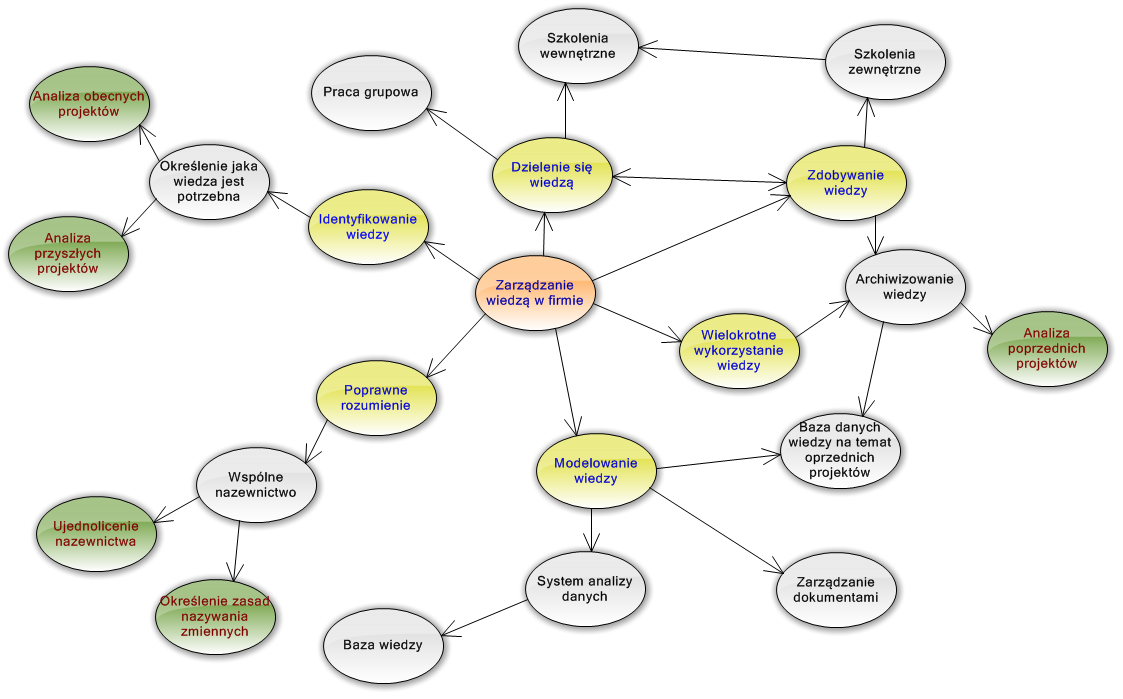
\includegraphics[width=0.6\textwidth]{mapaMysli.png}
\caption{Mapa myśli}
\label{fig:mapaMysli}
\end{figure}

% ===========================================================================

\section{Przegląd praktyk OPM3}
% strona 89

Ten wirtualny warsztat jest beznadziejny.


